\documentclass{article}

\def\npart{III}
\def\nyear{2018}
\def\nterm{Michaelmas}
\def\nlecturer{Professor I.\ Smith}
\def\ncourse{Algebraic Topology}
\def\draft{Ongoing course, rough}
\ifx \nauthor\undefined
  \def\nauthor{Bhavik Mehta}
\else
\fi

\author{Based on lectures by \nlecturer \\\small Notes taken by \nauthor}
\date{\nterm\ \nyear}
\title{Part \npart\ -- \ncourse}

\usepackage[utf8]{inputenc}
\usepackage{amsmath}
\usepackage{amsthm}
\usepackage{amssymb}
\usepackage{enumerate}
\usepackage{mathtools}
\usepackage{graphicx}
\usepackage[dvipsnames]{xcolor}
\usepackage{tikz}
\usepackage{wrapfig}
\usepackage{centernot}
\usepackage{float}
\usepackage{braket}
\usepackage[hypcap=true]{caption}
\usepackage{enumitem}
\usepackage[colorlinks=true, linkcolor=mblue]{hyperref}
\usepackage[nameinlink,noabbrev]{cleveref}
\usepackage{nameref}
\usepackage[margin=1.5in]{geometry}

% Theorems
\theoremstyle{definition}
\newtheorem*{aim}{Aim}
\newtheorem*{axiom}{Axiom}
\newtheorem*{claim}{Claim}
\newtheorem*{cor}{Corollary}
\newtheorem*{conjecture}{Conjecture}
\newtheorem*{defi}{Definition}
\newtheorem*{eg}{Example}
\newtheorem*{ex}{Exercise}
\newtheorem*{fact}{Fact}
\newtheorem*{law}{Law}
\newtheorem*{lemma}{Lemma}
\newtheorem*{notation}{Notation}
\newtheorem*{prop}{Proposition}
\newtheorem*{question}{Question}
\newtheorem*{rrule}{Rule}
\newtheorem*{thm}{Theorem}
\newtheorem*{assumption}{Assumption}

\newtheorem*{remark}{Remark}
\newtheorem*{warning}{Warning}
\newtheorem*{exercise}{Exercise}

% \newcommand{\nthmautorefname}{Theorem}

\newtheorem{nthm}{Theorem}[section]
\newtheorem{nlemma}[nthm]{Lemma}
\newtheorem{nprop}[nthm]{Proposition}
\newtheorem{ncor}[nthm]{Corollary}
\newtheorem{ndef}[nthm]{Definition}

% Special sets
\newcommand{\C}{\mathbb{C}}
\newcommand{\N}{\mathbb{N}}
\newcommand{\Q}{\mathbb{Q}}
\newcommand{\R}{\mathbb{R}}
\newcommand{\Z}{\mathbb{Z}}

\newcommand{\abs}[1]{\left\lvert #1\right\rvert}
\newcommand{\norm}[1]{\left\lVert #1\right\rVert}
\renewcommand{\vec}[1]{\boldsymbol{\mathbf{#1}}}

\let\Im\relax
\let\Re\relax

\DeclareMathOperator{\Im}{Im}
\DeclareMathOperator{\Re}{Re}
\DeclareMathOperator{\id}{id}

\definecolor{mblue}{rgb}{0., 0.05, 0.6}


% preamble

\setcounter{section}{-1}

\DeclarePairedDelimiter\ceil{\lceil}{\rceil}
\DeclarePairedDelimiter\floor{\lfloor}{\rfloor}
\DeclareMathOperator{\image}{image}
\DeclareMathOperator{\im}{im}

%\newtheorem{manualtheoreminner}{Theorem}
%\newenvironment{manualtheorem}[1]{%
%    \renewcommand\themanualtheoreminner{#1}%
%    \manualtheoreminner
%}{\endmanualtheoreminner}

%\newcommand{\red}[1]{\textcolor{bred}{#1}}
%\newcommand{\green}[1]{\textcolor{bgreen}{#1}}
%\newcommand{\blue}[1]{\textcolor{bblue}{#1}}
%\newcommand{\yellow}[1]{\textcolor{byellow}{#1}}
%\newcommand{\orange}[1]{\textcolor{borange}{#1}}
%\newcommand{\purple}[1]{\textcolor{bpurple}{#1}}

% and here we go!

\begin{document}
\maketitle

\tableofcontents

\clearpage
\section{Introduction}
Algebraic topology concerns the connectivity properties of topological spaces.
Recall a space $X$ is \textbf{connected} if we cannot write $X = U \cup V$ where $U,V$ are non-empty, open and disjoint.
\begin{eg}
  $\mathbb{R}$ is connected (with its Euclidean topology), $\mathbb{R} \setminus \{0\}$ is not connected.
\end{eg}

\begin{cor}[Intermediate value theorem]
  If $f: \mathbb{R} \to \mathbb{R}$ is continuous and $f(x)>0, f(y) < 0$, then there is some $z$ lying between $x,y$ such that $f(z) = 0$.
\end{cor}
\begin{proof}
  If $f(z) \neq 0$ for all $z$, then $\mathbb{R} = f^{-1}(-\infty,0) \cup f^{-1}(0, \infty)$ is disconnected.
\end{proof}
For nice spaces, connected $\iff$ path-connected.
Recall: a space $X$ is path-connected if $\forall x,y \in X, \exists \gamma:[0,1] \to X$ continuous such that $\gamma(0) = x, \gamma(1) = y$.
Informally, any two maps of a point to $X$ can be continuously deformed into one another.
\begin{center}
  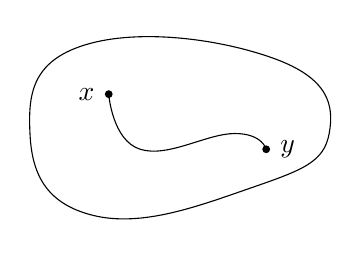
\begin{tikzpicture}[xscale=2]
    \draw plot [smooth cycle, tension=0.8] coordinates {(-180:1) (-120:1.2) (-60:0.8) (0:0.9) (60:1.1) (120:1.3)};
    \draw plot [smooth, tension=0.8] coordinates {(-0.5,0.5) (-0.3,-0.2) (0.3, 0) (0.5,-0.2)};
    \node [fill=black, circle, inner sep=1pt, label=left:$x$] at (-0.5,0.5) {};
    \node [fill=black, circle, inner sep=1pt, label=right:$y$] at (0.5,-0.2) {};
  \end{tikzpicture}
\end{center}
\begin{defi}[Homotopy]
  If $X,Y$ are topological spaces and $f,g : X \to Y$ are (continuous) maps, then $f$ is \textbf{homotopic} to $g$ if
  \begin{equation*}
    \exists F: X \times [0,1] \to Y
  \end{equation*}
  continuous such that
  \begin{equation*}
    F|_{X \times \{0\}} = f,
    F|_{X \times \{1\}} = g.
  \end{equation*}
  Write $f \simeq g$ or $f \simeq_F g$ and schematically
  \begin{center}
    \begin{tikzpicture}[scale=2]
      \draw (0,0) rectangle (1,1);
      \node at (0.5, 0.5) {$F$};
      \node at (0.5, -0.1) {$f$};
      \node at (0.5, 1.1) {$g$};
      \node (0) at (-0.2, 0) {$0$};
      \node (1) at (-0.2, 1) {$1$};
      \draw [->] (0) -- (1);
    \end{tikzpicture}
  \end{center}
\end{defi}

\begin{defi}[Simply connected]
  A path-connected space $X$ is \textbf{simply connected} if every two continuous maps $S^1 \to X$ are homotopic.
  Here $S^n = \set{x \in \mathbb{R}^{n+1} | \|x\| = 1}$ is the $n$ dimensional sphere, $S^1$ is the circle $\subseteq \mathbb{C}$.
\end{defi}
\begin{eg}
  $\mathbb{R}^2$ is simply connected but $\mathbb{R}^2 \setminus \{0\}$ is not. In fact, continuous maps $S^1 \xrightarrow{\gamma} \mathbb{R}^2 \setminus \{0\}$ have a degree $\deg(\gamma) \in \mathbb{Z}$, invariant under homotopy.
  (If $\gamma$ was differentiable, we could set $\deg(\gamma) = \frac{1}{2\pi i} \int_\gamma \frac{dz}{z} \in \mathbb{Z}$.)
  If $\gamma_n: S^1 \to \mathbb{R}^2 \setminus \{0\}$ has $t \mapsto e^{2\pi int}$ then $\deg(\gamma_n) = n$.
\end{eg}
\begin{cor}[Fundamental theorem of algebra]
  Every nonconstant complex polynomial has a root.
\end{cor}
\begin{proof}
  Let $f(z) = z^n + a_1 z^{n-1} + a_2 z^{n-2} + \dotsb + a_n$ be a complex polynomial and suppose $f(z) \neq 0 \ \forall z \in \mathbb{C}$. Let $\gamma_R(t) = f(R e^{2\pi it})$ so $\gamma_R : S^1 \to \mathbb{R}^2 \setminus \{0\}$.
  Now $\gamma_0$ is a constant map, so $\deg(\gamma_0) = 0$. By homotopy invariance of degree, $\deg(\gamma_R) = 0 \ \forall R$.

  If $R \gg \sum_i |a_i|$, we can consider $f_s(z) = z^n + s(a_1 z^{n-1} + \dotsb + a_n)$ for $0 \leq s \leq 1$, and on the circle $R e^{2\pi i t}$, $f_s$ also takes values in $\mathbb{R}^2 \setminus \{0\}$.
  If $\gamma_{R,s}(t) = f_s(R e^{2 \pi i t})$, then $\gamma_{R,1} = \gamma_R$ but $\gamma_{R,0} : z \mapsto z^n$, which has degree $n$.
  Now $\deg(\gamma_0) = \deg(\gamma_R) = \deg(\gamma_{R,1}) = \deg(\gamma_{R,0})$, so $n=0$ and $f$ is constant.
\end{proof}
\begin{fact}
  Any two maps $S^n \to \mathbb{R}^{n+1}$ are homotopic but maps $S^n \xrightarrow{f} \mathbb{R}^{n+1} \setminus \{0\}$ have a degree $\deg(f) \in \mathbb{Z}$, invariant up to homotopy.
  Moreover, the degree of the constant map is $0$ and the degree of inclusion is $1$.
\end{fact}
\begin{cor}[Brouwer's fixed point theorem]
  If $B^n = \set{x \in \mathbb{R}^n | \|x\| \leq 1}$, any continuous map $f: B^n \to B^n$ has a fixed point.
\end{cor}
\begin{proof}
  Suppose $f$ has no fixed point.
  Let $\gamma_R: S^{n-1} \to \mathbb{R}^n \setminus \{0\}$ be the map $v \mapsto R_v - f(R_v)$ for $0 \leq R \leq 1$. So $\gamma_0$ is a constant, so has degree 0.
  Hence $\deg(\gamma_1) = 0$.

  Let $\gamma_{1,s}(v) \coloneqq v - s f(v)$, for $0 \leq s \leq 1$ and $v \in S^{n-1}$.
  Note $\gamma_{1,s}$ has image in $\mathbb{R}^n \setminus \{0\}$: if $s=1$, this is because $v \neq f(v) \ \forall v$ and if $s < 1$ then $|v| > |s f(v)|$.
  Therefore $\gamma_1 = \gamma_{1,1}$ has the same degree as $\gamma_{1,0}$ which is the inclusion $S^{n-1} \hookrightarrow \mathbb{R}^n\setminus\{0\}$, a contradiction.
\end{proof}
\begin{defi}[Homotopy equivalence]
  We say spaces $X,Y$ are \textbf{homotopy equivalent} if $\exists$ maps $f : X \to Y$ and $g: Y \to X$ such that $g \circ f \simeq \id_X$ and $f \circ g \simeq \id_Y$. We write $X \simeq Y$.
\end{defi}
\begin{eg}\leavevmode
  \begin{itemize}
    \item Trivial case: if $X,Y$ are homeomorphic, i.e.\ $X \cong Y$, then clearly $X \simeq Y$.

    \item $\mathbb{R}^n \simeq \{0\}$, the single point. A space homotopy equivalent to a point is sometimes called contractible.
    \item $\mathbb{R}^n \setminus \{0\} \simeq S^{n-1}$.
      If $i: S^{n-1} \hookrightarrow \mathbb{R}^n \setminus \{0\}$ inclusion, and $p: \mathbb{R}^n \setminus \{0\} \to S^{n-1}$ is projection $v \mapsto \frac{v}{\|v\|}$, then $p \circ i = \id_{S^{n-1}}$ and $i \circ p \simeq \id_{\mathbb{R}^n \setminus \{0\}}$ via the homotopy
      \begin{align*}
        F: \mathbb{R}^n \setminus \{0\} \times [0,1] &\longrightarrow \mathbb{R}^n \setminus \{0\} \\
        (v,t) &\longmapsto t v + (1-t) \frac{v}{\|v\|}
      \end{align*}
  \end{itemize}
\end{eg}
Algebraic topology is the study of the set of spaces up to homotopy equivalence via the set of groups up to isomorphism.

The first naive attempt would be homotopy groups:
Loops (continuous maps $S^1 \to X$) with a common base-point can be concatenated and this induces a group structure on the set of homotopy classes of maps $(S^1, *) \to (X, x_0)$.
This refers to continuous maps $S^1 \to X$ taking $* \mapsto x_0$ and a based homotopy $F : f \simeq g$ of two such is one such that $F |_{S \times \{t\}}$ sends $*$ to $x_0$ $\forall t$.

Again, there is a group structure on the set of based homotopy classes of maps $(S^n, *) \to (X, x_0)$ calld $\pi_n(X, x_0)$, the $n$-th homotopy group of $X$.
\begin{fact}
  $\{\pi_n(S^2, x)\}_{n \geq 1}$ is not known. Indeed, there is no simply connected manifold of dimension $> 0$ for which all $\pi_n$ are known.
\end{fact}

Instead, we will focus on homology theory, more precisely singular (co)homology.
We will obtain invariants of spaces in a two-step process:
\begin{enumerate}[label=(\alph*)]
  \item Associate to $X$ a chain complex (or cochain complex).
  \item take (co)homology of that complex.
\end{enumerate}
This will be rather computable for simple spaces. In this course, we will mostly focus on studying manifolds.
\begin{defi}[Chain complex, cochain complex]
  A \textbf{chain complex} $(C_*, d)$ is a sequence of abelian groups and homomorphisms
  \begin{equation*}
    \dots \longrightarrow C_{n+1} \overset{d_{n+1}}{\longrightarrow} C_n \overset{d_n}{\longrightarrow} C_{n-1} \overset{d_{n-1}}{\longrightarrow} C_{n-2} \longrightarrow \dots
  \end{equation*}
  (indexed by $\mathbb{N}$ or $\mathbb{Z}$) with the key property that $\forall n \ d_{n-1} \circ d_n = 0$
  Then $\image(d_{n+1}) \subseteq \ker(d_n)$ and the $n$-th homology group $H_n(C_*, d)$ of the chain complex is the quotient
  \begin{equation*}
    H_n(C_*, d) \coloneqq \frac{\ker(d_n)}{\im(d_{n+1})}.
  \end{equation*}

  A \textbf{cochain complex} $(C^*, d)$ is a sequence of abelian groups and homomorphisms
  \begin{equation*}
    \dots \longrightarrow C_{n+1} \overset{d_{n-1}}{\longrightarrow} C_n \overset{d_n}{\longrightarrow} C_{n+1} \longrightarrow \dots
  \end{equation*}
  such that $d^n \circ d^{n-1} \equiv 0 \ \forall n$
  The $n$-th cohomology group $H^n(C^*, d)$ is the quotient
  \begin{equation*}
    H^n(C^*, d) \coloneqq \frac{\ker(d^n)}{\im(d^{n-1})}.
  \end{equation*}
\end{defi}
\end{document}
